\chapter{Introduction}
\section{Braess' Paradox}
\begin{center}
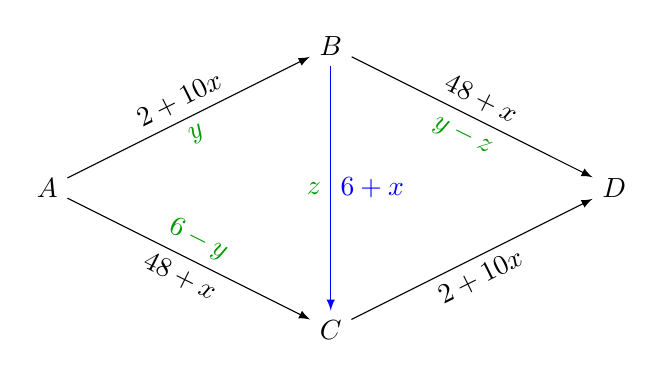
\begin{tikzpicture}[
    scale=0.9,               % 调整整体大小
    >={latex}
]

    % --- 1. 定义节点位置 (Nodes) ---
    \node (A) at (0, 0) {$A$};
    \node (B) at (4, 2) {$B$};
    \node (C) at (4, -2) {$C$};
    \node (D) at (8, 0) {$D$};

    % --- 2. 绘制黑色路径 (Black Edges) ---
    
    % A -> B (Top Left)
    % 黑色文字在上方，绿色流量 y 在下方
    \draw[->] (A) -- 
        node[above, sloped] {$2+10x$} 
        node[below, sloped, text=green!60!black] {$y$} 
        (B);

    % A -> C (Bottom Left)
    % 黑色文字在下方，绿色流量 6-y 在上方 (原图中写的是 6-y 或 b-y，此处按流量守恒推断为 6-y)
    \draw[->] (A) -- 
        node[below, sloped] {$48+x$} 
        node[above, sloped, text=green!60!black] {$6-y$} 
        (C);

    % B -> D (Top Right)
    % 黑色文字在上方，绿色流量 y-z 在下方
    \draw[->] (B) -- 
        node[above, sloped] {$48+x$} 
        node[below, sloped, text=green!60!black] {$y-z$} 
        (D);

    % C -> D (Bottom Right)
    % 黑色文字在下方 (原图中这部分似乎没有标绿色流量，如果需要可以加上)
    \draw[->] (C) -- 
        node[below, sloped] {$2+10x$} 
        (D);

    % --- 3. 绘制蓝色捷径 (Blue Shortcut) ---
    
    % B -> C (Middle)
    % 蓝色箭头，右侧标成本，左侧标绿色流量 z
    \draw[->, blue] (B) -- 
        node[right] {$6+x$} 
        node[left, text=green!60!black] {$z$} 
        (C);

\end{tikzpicture}
\end{center}

The core idea to solve for equilibrium is that, in equilibrium costs (the time spent on each possible route from $A$ to $D$) on all paths must be equal. So one can show that before the shortcut is connected, the equilibrium travel time for any driver is $83$ minutes. After the shortcut is built, the new equilibrium travel time becomes $92$, which is actually greater than the original one.

In the example, although the network capacity increased by adding the shortcut, the individual cost for every agent increased. This is due to the negative externality: when an agent switches to the shortcut, they reduce their own time marginally but impose a heavy congestion cost on the shared links $AB$ and $CD$. This cost is not internalized by the selfish agent. 

\rmkb{
  \begin{itemize}
    \item In a multi-agent situation, having more choices can possibly make you (and even everyone) worse off. 
    \item However in single-person situations, having more choices will make you at least as well off.
  \end{itemize}
}

\section{Coin Toss}

Agent A announces her guess first, and then B announces her guess after observing A's guess. If both agents make the same guess, then both agents get 1. Otherwise, nature determines the winner by coin toss. Whoever's guess matches the coin toss wins 4 and the other gets 0.
\[
\begin{array}{cccc}
\text{Coin} & A & B & \text{Payoff} \\
\hline
H & H & H & (1,1) \\
T & H & H & (1,1) \\
H & T & T & (1,1) \\
T & T & T & (1,1) \\
H & H & T & (4,0) \\
H & T & H & (0,4) \\
T & H & T & (0,4) \\
T & T & H & (4,0) \\
\end{array}
\]

If the coin toss is unavailable to both of them, B will make a guess opposite to $A$'s as long as $B$ is not too risk averse. Hence the expected payoff is $(2,2)$.

If the coin toss is made available to $A$, and this rule is common knowledge, the best strategy for $A$ is to make a guess consistent with the actual coin toss, and $B$'s best response is to report the same as $A$. Hence both will get a certain payoff $(1,1)$.

\rmkb{
  Information can indeed have a negative value! In the example, if the revelation of coin toss to $A$ is made a common knowledge, this information can actually make $A$ worse off. However if the revelation is $A$'s private knowledge, then it must have nonnegative value.
}

\section{Model of Herding}

Suppose there are two restaurants in the town, $A$ and $B$. The common prior is that 
\[
\Pr{A>B} = p>\frac{1}{2},
\]
where $A>B$ denotes the event that restaurant $A$ is better than $B$. This common prior states that everyone is inclined to choose $A$ if there is no other informative signal. Suppose there are two types of signals, $\alpha$ and $\beta$, such that
\[
\begin{aligned}
  \Pr{\alpha|A>B} = q,\\
  \Pr{\beta|B>A} = q,
\end{aligned}
\]
where $q>\frac{1}{2}$ and $q>p$\footnote{
  $q>p$ ensures that an agent observing a signal contrary to the prior will form a posterior belief that favors the signal over the prior.
}.

The $t$-th agent knows all $(t-1)$ prior agents' choices, but does not know their private signals. 

Suppose the signal sequence is $(\alpha,\beta,\beta,\cdots,\beta)$.

For Agent 1, she receives signal $\alpha$, which enhances the prior through Bayesian updating. Since $\Pr{A>B|\alpha} > \frac{1}{2}$, she chooses $A$. 

For Agent 2, she deduces from Agent 1's choice to infer that Agent 1 must have received signal $\alpha$. But Agent 2's private signal is $\beta$. Nevertheless, the two signals cancel out\footnote{
  This can be rigorously verified using Bayes' rule:
  \[
  \begin{aligned}
    \Pr{A>B|\alpha,\beta} &= \frac{\Pr{\alpha,\beta|A>B}\Pr{A>B}}{\Pr{\alpha,\beta|A>B}\Pr{A>B} + \Pr{\alpha,\beta|B>A}\Pr{B>A}}\\
    &= \frac{q(1-q) \cdot p}{q(1-q) \cdot p + (1-q)q \cdot (1-p)}\\
    &= p > \frac{1}{2}.
  \end{aligned}
  \]
  Thus, observing signals $\alpha$ (inferred from Agent 1) and $\beta$ (private) leaves Agent 2's posterior identical to the prior, as if she had received no informative evidence.
}. Hence, the common prior dictates that Agent 2 should also choose $A$.

For Agent 3, she deduces that Agent 1 must have received signal $\alpha$ from Agent 1's choice. Regarding Agent 2, Agent 3 reasons as follows: if Agent 2 received $\alpha$, then Agent 2 would vote for $A$; if Agent 2 received $\beta$, then the two signals cancel out and Agent 2 still chooses $A$ by the prior. Therefore, Agent 2's choice is uninformative about the true state. Hence, Agent 3 only infers the informative signal $s_1 = \alpha$ from history, and combined with her own signal $s_3 = \beta$, the two signals cancel out, leading Agent 3 to also choose $A$.

The same logic applies to all the subsequent agents. Hence, all agents choose $A$ regardless of their private signals. This is the herding phenomenon.

\rmkb{
  \begin{itemize}
    \item The assumption that $q>p$ is important because it ensures that
  \[
  \begin{aligned}
    \Pr{B>A|\beta} & = \frac{\Pr{\beta|B>A}\Pr{B>A}}{\Pr{\beta|B>A}\Pr{B>A} + \Pr{\beta|A>B}\Pr{A>B}} \\
    & = \frac{q(1-p)}{q(1-p)+(1-q)p}>\frac{1}{2}.
  \end{aligned}
  \]
  Similarly, you can verify that $\Pr{A>B|\alpha}>\frac12$.

  So this assumption implies that private signals are sufficiently informative to overturn the prior. Specifically, it ensures that an agent observing a signal contrary to the prior will form a posterior belief that favors the signal over the prior. Otherwise, the agent will be ``blinded'' by the prior.
    \item Even though the signal is strong enough to overturn the prior, the information cascade is not perfect. Starting from Agent 2, the information cascade breaks.
  
    \item Agent $2$ only cares about maximizing their own payoff. If Agent $2$ also cared about social welfare, they would choose according to their private signal (choose $B$ if they get $\beta$) to reveal their information to Agent $3$ and subsequent agents. However, there is no individual incentive to do so, making this an information externality that leads to inefficiency.
  \end{itemize}
}

